\subsubsection{Background}
The Corporate Partnership Program is a website designed to `promote the relationship between the Department of Computing and organisations who wish to recruit our students whilst investing in academic sponsorship'\cite{doc-cpp}.

In order for students to use the system they must log on, register some tick box interests, and then upload their CV.
For the student once they have done this their CPP journery is complete.
Coporate Partnets then log on, and can browse this list of students in order to contact them regarding internships, placements, and graduate oppourtunities.

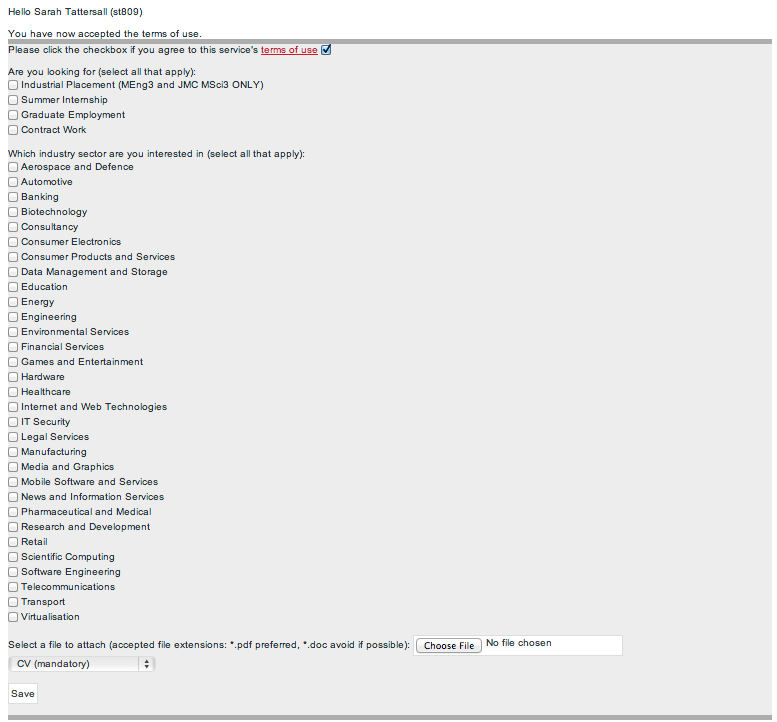
\includegraphics[scale=0.5]{images/introduction/old_cpp}

However as you can see from the picture above the system is very out dated and does not freely allow a student to express their interests and skills. Furthermore companies have no way of viewing a students skills before looking at their CV. This means that companies must go through every student listed in the database whilst searching for one with particular skills. For example a web development company may only wish to recruit summer interns who have experience with Ruby on Rails. On the current system they must download every single students CV in turn to ascertain if a student has this skill, something which is time consuming, frustrating, and realistically is unlikely to happen.
This can severly disadvantage students whose CV's appear at the bottom of the list and unfortunately students have
no way of making themselves better found.

The current system has other flaws, for example once it's been set up there is no way for administrators to tell which corporate partners are using the system and how many students are being contacted. What goes on with the system is really a black hole to the Department of Computing Industrial Liaison Officers. 

Other departments have expressed an interest in this system, however it is not deemed up to date enough to pass on to another department.